\documentclass[12pt]{article}
\usepackage{amsmath,amssymb,graphicx}
\usepackage{float}
\usepackage{caption}
\usepackage{geometry}
\geometry{a4paper, margin=1in}

\title{Charge Pumps}
\author{}
\date{}

\begin{document}

\maketitle

\section{Introduction to Charge Pumps}
A charge pump is a circuit that sources or sinks charge for a controlled amount of time. A simple realization is: if $S_1$ is on, $I_1$ charges $C_1$, and if $S_2$ is on, $I_2$ discharges it.

\begin{figure}[H]
    \centering
    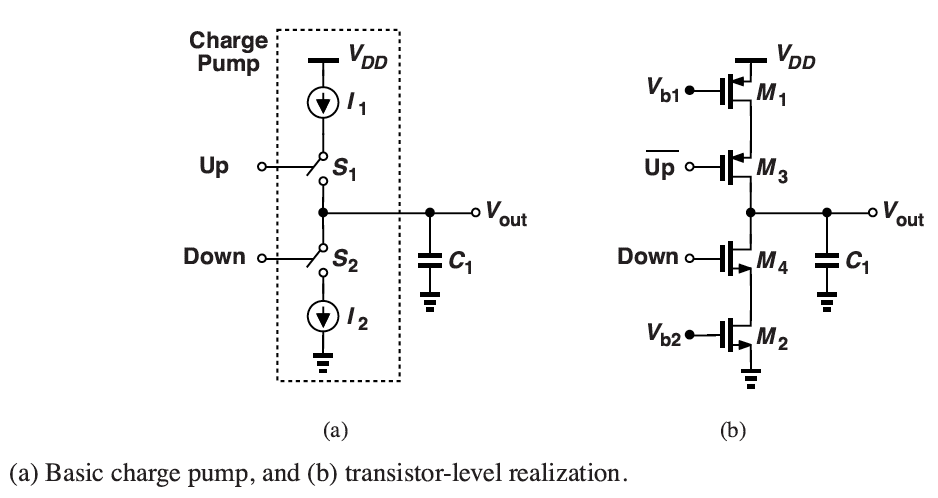
\includegraphics[width=0.6\textwidth]{figs/cp1}
    \caption{Basic charge pump circuit}
\end{figure}

The controls are called \textbf{Up} and \textbf{Down}, respectively, determining whether the output voltage rises or falls. Assume $I_1 = I_2 = I_p$. The transistor-level implementation uses $M_1$ and $M_2$ as current sources and $M_3$ and $M_4$ as switches. This is called a “drain-switched” CP.

\section{CP/Capacitor Cascade}
Each time a phase comparison is made, $QA$ goes high, $S_1$ turns on, $I_1$ charges $C_1$, and $V_{out}$ rises by:
\[
\Delta V = \left(\frac{I_p}{C_1}\right)\Delta T
\]

\begin{figure}[H]
    \centering
    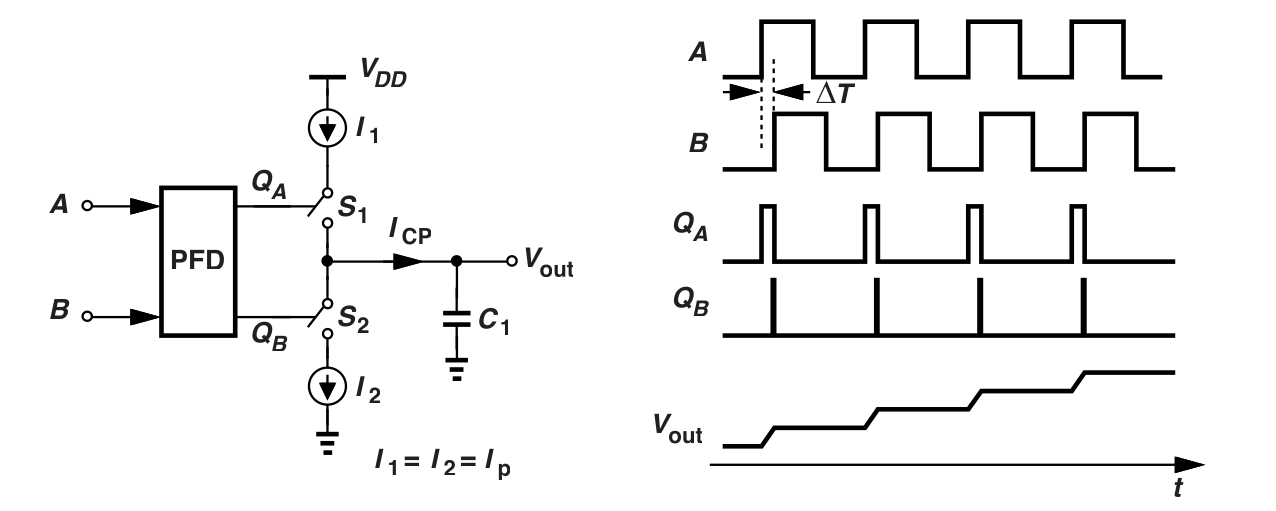
\includegraphics[width=0.6\textwidth]{figs/cp2}
    \caption{CP/Capacitor cascade operation}
\end{figure}

If the phase difference remains constant, $V_{out}$ increases indefinitely, implying infinite gain for finite phase error. For $V_{out}$ to be finite, the phase error must be zero.

\section{Basic Charge-Pump PLL}
We now construct a PLL using the PFD/CP/capacitor cascade. If the loop is locked:
\[
f_{out} = f_{in}, \quad \phi_{out} = \phi_{in}
\]

\begin{figure}[H]
    \centering
    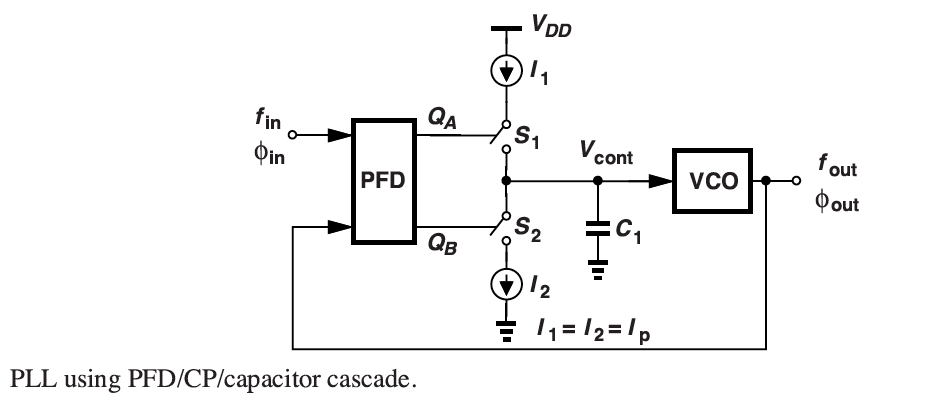
\includegraphics[width=0.7\textwidth]{figs/cp3}
    \caption{PLL using PFD/CP/capacitor cascade}
\end{figure}

The loop locks with zero static phase error due to the integration effect of the CP and capacitor.

\section{CP Transfer Function}
The impulse response is derived by first applying a phase step. The voltage change each cycle is:
\[
\Delta V = \left(\frac{\Delta \phi_1}{2\pi}\right)T_{in}\left(\frac{I_p}{C_1}\right)
\]
The slope is:
\[
\frac{\Delta V}{T_{in}} = \left(\frac{\Delta \phi_1}{2\pi}\right)\left(\frac{I_p}{C_1}\right)
\]
Thus, the impulse response is:
\[
h(t) = \left(\frac{\Delta \phi_1}{2\pi}\right)\left(\frac{I_p}{C_1}\right)u(t)
\]
And the Laplace transform (transfer function):
\[
\frac{V_{cont}(s)}{\Delta \phi(s)} = \frac{I_p}{2\pi C_1 s}
\]

\begin{figure}[H]
    \centering
    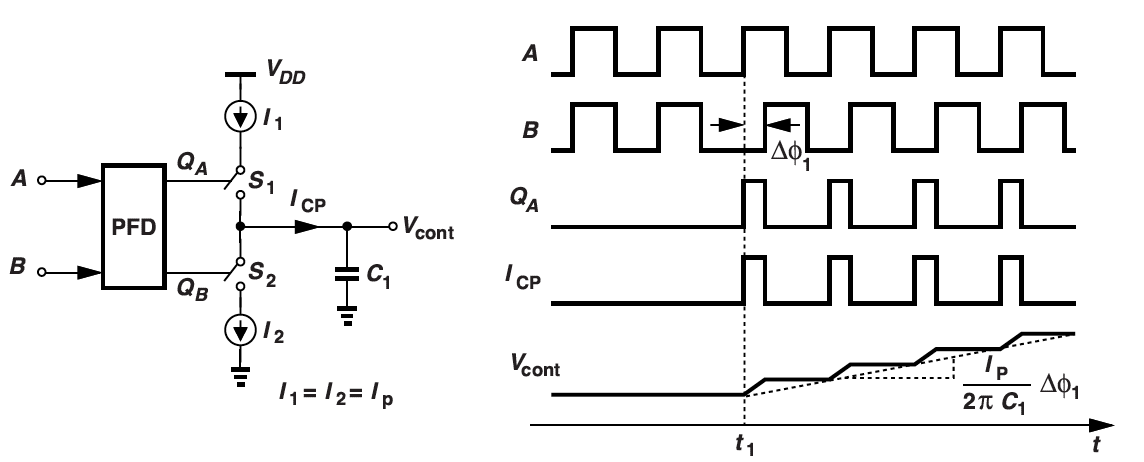
\includegraphics[width=0.65\textwidth]{figs/cp4}
    \caption{Impulse response analysis of charge pump}
\end{figure}

This is an ideal integrator. Combined with a VCO having $K_{VCO}/s$, the open-loop transfer function is:
\[
H_{open}(s) = \frac{I_p K_{VCO}}{2\pi C_1 s^2}
\]
This has two poles at origin (type-II PLL), and the closed-loop transfer function is:
\[
H(s) = \frac{I_p K_{VCO}}{2\pi C_1 s^2 + I_p K_{VCO}}
\]

\section{Stabilizing the Loop}
To stabilize, a resistor $R_1$ is added in series with $C_1$:
\[
\frac{V_{cont}(s)}{\Delta \phi(s)} = \frac{I_p}{2\pi} \left( \frac{1}{C_1 s} + R_1 \right)
\]

\begin{figure}[H]
    \centering
    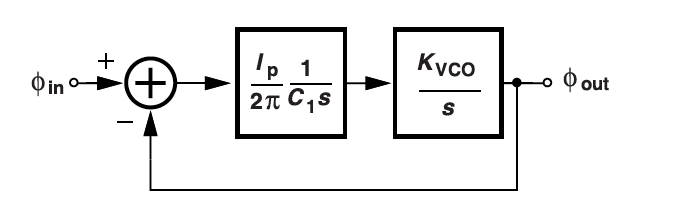
\includegraphics[width=0.65\textwidth]{figs/cp5}
    \caption{Stabilized loop with series resistor}
\end{figure}

The loop filter introduces a zero at $s = -1/(R_1 C_1)$. The closed-loop transfer function becomes:
\[
H(s) = \frac{I_p K_{VCO}}{2\pi C_1 (R_1 C_1 s + 1) s^2 + I_p K_{VCO} R_1 s + \frac{I_p K_{VCO}}{2\pi C_1}}
\]

With:
\[
\omega_n = \sqrt{\frac{I_p K_{VCO}}{2\pi C_1}}, \quad \zeta = \frac{R_1}{2} \sqrt{\frac{2\pi}{I_p K_{VCO} C_1}}
\]

\section{Real-World Considerations}
Charge pumps exhibit ripple on control voltage requiring additional capacitance.

\begin{figure}[H]
    \centering
    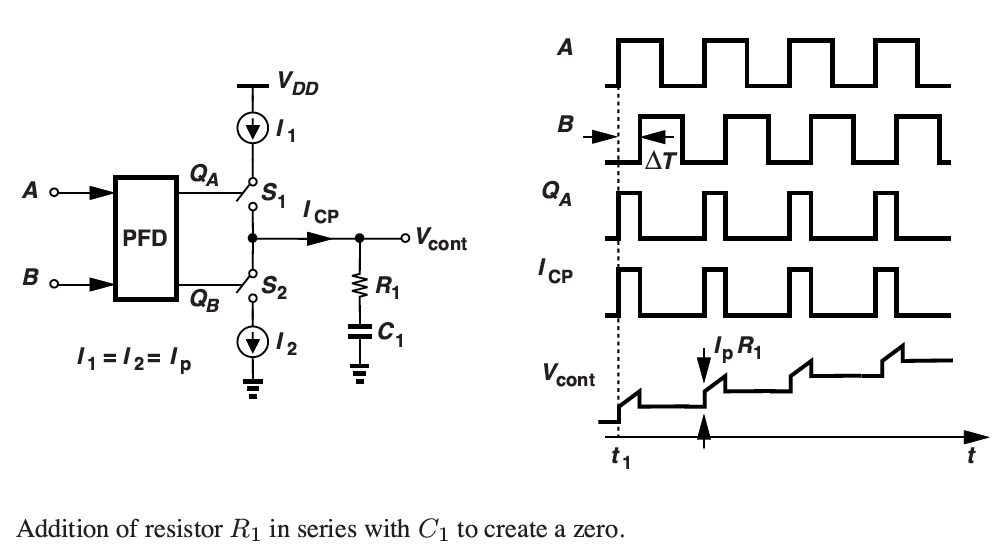
\includegraphics[width=0.65\textwidth]{figs/cp6}
    \caption{Skew and ripple effects in CP}
\end{figure}

Due to skew in control signals, current imbalance results in jumps in $V_{cont}$:
\[
\Delta V = \pm I_p R_1
\]

These jumps modulate the VCO:
\[
V_{out}(f) = j\frac{K_{VCO} I_p R_1 T_{sk} \Delta T}{T_{in}} \sum_{k=-\infty}^{\infty} \delta(f - M f_{in} - k f_{in})
\]

\section{Loop Filter Impedance and PM}
Add a second capacitor $C_2$. Impedance becomes:
\[
Z(s) = \left[R_1 + \frac{1}{C_1 s} \right] \parallel \left[ \frac{1}{C_2 s} \right]
\]

\begin{figure}[H]
    \centering
    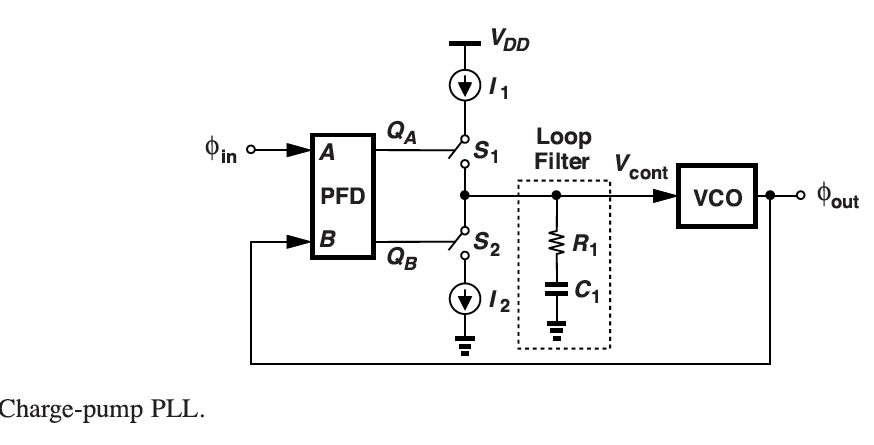
\includegraphics[width=0.6\textwidth]{figs/cp7}
    \caption{Loop filter with additional capacitor}
\end{figure}

\[
T(s) = \frac{I_p}{2\pi} \cdot \frac{R_1 C_1 s + 1}{R_1 C_{eq} s + 1} \cdot \frac{1}{(C_1 + C_2)s} \cdot \frac{K_{VCO}}{Ms}
\]

Where $C_{eq} = \frac{C_1 C_2}{C_1 + C_2}$ and third pole:
\[
\omega_{p3} = \frac{1}{R_1 C_{eq}}
\]

\begin{figure}[H]
    \centering
    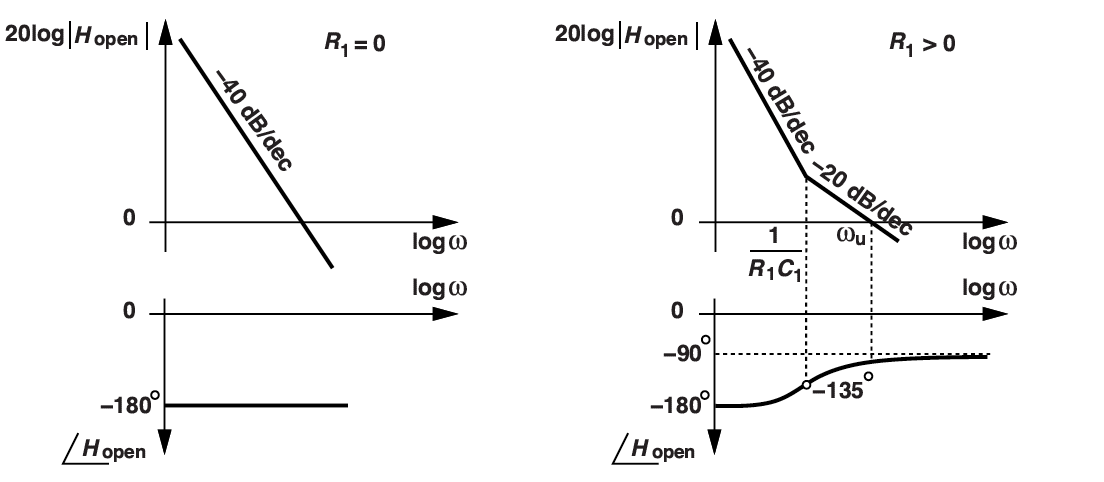
\includegraphics[width=0.6\textwidth]{figs/cp8}
    \caption{Phase margin response}
\end{figure}

Phase margin degradation:
\[
PM = \tan^{-1}(R_1 C_1 \omega_u) - \tan^{-1}(R_1 C_{eq} \omega_u)
\]

\section{Second-Order Filter Topology}
A second-order filter allows $V_{R_1}$ to jump, while $C_2$ smooths ripple.

\begin{figure}[H]
    \centering
    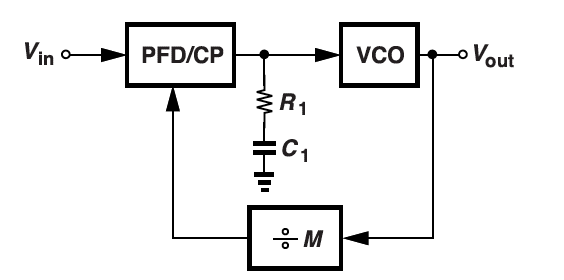
\includegraphics[width=0.65\textwidth]{figs/cp9}
    \caption{Second-order filter topology}
\end{figure}

If $C_1 \gg C_2$, $V_{cont}$ changes minimally during CP pulse. Then $C_2$ shares charge with $C_1$, stabilizing the loop.

\begin{figure}[H]
    \centering
    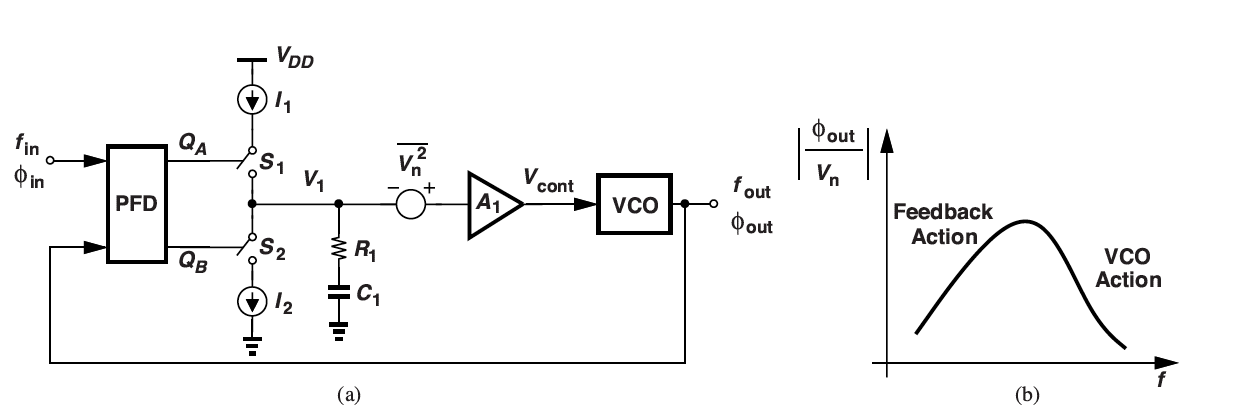
\includegraphics[width=0.6\textwidth]{figs/cp10}
    \caption{Charge sharing and pulse formation}
\end{figure}

\end{document}
